% meta.concepts: truss
% meta.tags: realistic
% acknowledge: Peter Seiler & Luke Melander graciously shared Spring 2019 course material
% source: 2019 P. Seiler AEM2011 HW 8

The Stone Arch Bridge in Minneapolis consists of 21 stone arch spans and one steel truss span. The steel truss
span replaced two of the original stone arches when the St. Anthony Falls lock and dam system was built.
Under maximum loading conditions, the truss experiences the forces shown in the diagram below. Assume
that:
\begin{itemize}
  \item horizontal members can withstand a maximum of 3600 kN in tension and 1200 kN in compression
  \item diagonal members can withstand a maximum of 1200 kN in tension and 400 kN in compression
  \item vertical members can withstand a maximum of 300 kN in tension and 100 kN in compression.
\end{itemize}

Find the value of $P_{max}$ such that the forces remain within the specified tension and compression limits. The truss is attached
to the bridge with a fixed support at A and a roller support at B.

\begin{figure}[ht!]
  \centering
  \includegraphics[width=0.4\textwidth,
	           height=0.4\textheight,
		   keepaspectratio]{figa.png}
  \includegraphics[width=0.4\textwidth,
	           height=0.4\textheight,
		   keepaspectratio]{figb.png}
  \caption*{Stone Arch Bridge (left) and free body diagram of steel truss span (right)}
\end{figure}

\iftoggle{flagSoln}{%
\vspace{.5cm}
\rule{\textwidth}{.4pt}
\vspace{.5cm}
\textbf{Solution:}
\begin{figure}[ht!]
  \centering
  \includegraphics[width=0.9\textwidth,
	           height=0.3\textheight,
		   keepaspectratio]{solna.png}
  \includegraphics[width=0.9\textwidth,
	           height=0.3\textheight,
		   keepaspectratio]{solnb.png}
  \includegraphics[width=0.9\textwidth,
	           height=0.3\textheight,
		   keepaspectratio]{solnc.png}
  \includegraphics[width=0.9\textwidth,
	           height=0.3\textheight,
		   keepaspectratio]{solnd.png}
  \includegraphics[width=0.9\textwidth,
	           height=0.3\textheight,
		   keepaspectratio]{solne.png}
  \includegraphics[width=0.9\textwidth,
	           height=0.3\textheight,
		   keepaspectratio]{solnf.png}
  \includegraphics[width=0.9\textwidth,
	           height=0.3\textheight,
		   keepaspectratio]{solng.png}
\end{figure}
}{%
}%
